\documentclass[11pt]{article}


% Packages
\usepackage{amsmath}
\usepackage{graphicx}
\usepackage{float}
\usepackage{listings}
\usepackage[font=small]{caption}
\usepackage{comment}
\usepackage[linesnumbered,vlined]{algorithm2e}
\usepackage{hhline}
\usepackage{geometry}
\usepackage{tabularx}
\usepackage{hyperref}
\usepackage{algorithm}

\graphicspath{./Images} 
% Layout settings
\renewcommand{\contentsname}{Index}
\renewcommand{\figurename}{Figure}
\renewcommand{\tablename}{Table}
\SetAlgoCaptionSeparator{}
\geometry{
    bottom=2.8cm
}

% Style
\lstdefinestyle{mystyle}{
    basicstyle=\ttfamily\footnotesize,
    breakatwhitespace=false,
    breaklines=true,
    captionpos=b,
    keepspaces=true,
    numbers=left,
    numbersep=5pt,
    showspaces=false,
    showstringspaces=false,
    showtabs=false,
    tabsize=2
}
\lstset{style=mystyle}

% Document intestation
\title{Confronto Order Statistics}
\author{Alessandro Aldo Raoul Bonciani}
\date{Aprile 2024}

\begin{document}
 \newgeometry{top=1.7cm, bottom=2.8cm}

\maketitle
\tableofcontents


\newpage
\section{Introduction}
\subsection{Description of the problem}
In this report we are going to compare the different implementations regarding dynamic order statistics of these data structures:
\begin{itemize}
    \item BST without the size attribute
    \item Ordered List
\end{itemize}
\subsection{Test technical specs}
The tests are all executed on the same machine, which runs on:\begin{itemize}
    \item \textbf{Processor:} Intel Core i7-7700HQ 2.80 GHz,
    \item \textbf{RAM:} 16.0 GB
    \item \textbf{Operating System:} Ubuntu 22.04.4 LTS
\end{itemize}
The code has been written and executed on Visual Studio Code (1.88.1) while this report has been written online using \textbf{\href{https://overleaf.com}{OverLeaf}}
\section{The data structures}
\subsection{Sorted List}
A sorted list is a data structure that maintains its elements in a particular order, typically either in ascending or descending order. This arrangement allows for efficient searching, insertion, and deletion operations. When new elements are added to a sorted list, they are inserted into the appropriate position to maintain the sorted order. Similarly, when elements are removed, the list adjusts to maintain the order. 
\subsection{BST}
A \textbf{B}inary \textbf{S}earch \textbf{T}ree is a kind of binary tree in which each vertex can have up to two children. This structure adheres to the BST property, stipulating that every vertex in the left subtree of a given vertex must carry a value smaller than that of the given vertex, and every vertex in the right subtree must carry a value larger. To go through this data structure, we use the \textit{inorderTreeWalk} method that works recursively. There are two versions for this method, one each for OS algorithm.
\section{Order Statistics}
Dynamic order statistics are a class of problems that require efficiently maintaining and querying a sequence of sorted elements. The OS-Select and OS-Rank algorithms are two operations of fundamental importance in this context:
\begin{itemize}
    \item \textbf{OS Select(k)} allows finding the k-th smallest element in a sequence, returning its pointer. 
    \item \textbf{OS Rank(x) }determines the position of an element x in the sorted sequence, returning the index.
\end{itemize}
\subsection{Order statistics in Sorted lists}
The OS Select algorithm for sorted lists has been implemented as follows: the list is traversed from the head until reaching the k-th element, which is returned by the function (if k exceeds the length of the list, a null value is returned).

For the OS Rank algorithm, a similar approach is taken: the list is traversed, comparing each node with the input node x provided to the function, while keeping track of how many nodes have been analyzed. Once the node x is found, the function outputs its position in the sorted sequence (or returns 0 if x does not belong to the list).
\subsubsection{Pseudocodes}
\begin{algorithm}[H] 
\SetAlgoLined
\KwIn{An integer $i$}
\KwOut{Node at the $i$-th position in the list}
\vspace{0.5em}
\captionabove{\underline{OS\_Select(i)}} \\
\vspace{0.5em}
$j \leftarrow 1$\\
$tmpNode \leftarrow \text{self.head}$\\
\While{$tmpNode \neq \text{None} \land j \neq i$}{
    $j \leftarrow j + 1$\\
    $tmpNode \leftarrow tmpNode.next$\\
}
\Return $tmpNode$
\end{algorithm}
\vspace{1em}
\begin{algorithm}[H] 
\SetAlgoLined
\KwIn{A $node$}
\KwOut{The rank of the $node$ in the $List$}
\vspace{0.5em}
\captionabove{\underline{OS\_Rank($node$)}} \\
\vspace{0.5em}
$tmpNode \leftarrow \text{self.head}$\\
$i \leftarrow 1$\\
\While{$tmpNode \neq \text{None} \land tmpNode.key \neq \text{node.key}$}{
    $tmpNode \leftarrow tmpNode.next$\\
    $i \leftarrow i + 1$\\
}
\If{$tmpNode \text{ è None}$}{
    $i \leftarrow 0$\\
}
\Return $i$
\end{algorithm}


\vspace{0.0em}
\subsection{Order statistics in BST}
Regarding the binary search tree, the operation is entirely analogous to that of sorted lists, with the only difference being that the tree is traversed not sequentially but through the inorderTreeWalk method, which operates recursively. There are two versions of this method, one for the OS algorithm, which differ in their termination criteria.
\subsubsection{Pseudocodes}
\begin{algorithm}[H] 
\SetAlgoLined
\KwIn{An integer $i$}
\KwOut{Node at the $i$-th position in the BST}
\vspace{0.5em}
\captionabove{\underline{OS\_Select(i)}} \\
\vspace{0.5em}
$\text{self.osCounter} \leftarrow 1$\\
$\text{self.\_\_inorderTreeWalkSelect(self.root, i)}$\\
$\text{self.osCounter} \leftarrow 0$\\
$\text{self.found} \leftarrow \text{False}$\\
$x \leftarrow \text{self.rankedNode}$\\
$\text{self.rankedNode} \leftarrow \text{None}$\\
\Return $x$
\end{algorithm}

\vspace{1em}

\begin{algorithm}[H] 
\SetAlgoLined
\KwIn{A $node$}
\KwOut{The rank of the $node$ in the BST}
\vspace{0.5em}
\captionabove{\underline{OS\_Rank(node)}} \\
\vspace{0.5em}
$\text{self.osCounter} \leftarrow 1$\\
$\text{self.\_\_inorderTreeWalkRank(self.root, node)}$\\
$i \leftarrow \text{self.osCounter}$\\
$\text{self.osCounter} \leftarrow 0$\\
$\text{self.found} \leftarrow \text{False}$\\
\If{$i > \text{self.size}$}{
    $i \leftarrow 0$\\
}
\Return $i$
\end{algorithm}
\section{Differences beetween the data structures}
For what concerns the \textit{OS\_Rank} algorithm, there are these main differences:
\begin{table}[H]
                \centering
                \begin{tabular}{|c|c|}
                    \hline
                    \textbf{Data Structure} & \textbf{Time complexity} \\
                    \hline
                    List & {$O(n)$} \\
                    \hline
                    BST & {$O(n + \log n)$} \\
                    \hline
                    \end{tabular}
                \caption{OS\_Rank time complexity.}
\end{table}
Explained as follows:
\begin{itemize}
    \item \textbf{List:} The algorithm can traverse the list until it reaches the specified node and count the number of preceding nodes. Since the list is sorted, the algorithm can find the rank of the node in $O(n)$ operations, where $n$ is the size of the list.
    \item \textbf{BST:} The algorithm performs an in-order traversal of the binary search tree until it finds the specified node. After finding the node, it counts how many nodes precede the found node during the in-order traversal. Since an in-order traversal has a cost of $O(n)$ and searching for the node may require $O(\log n)$ operations in the worst case, the approximate cost of OS\_Rank is $O(n + \log n)$.
\end{itemize}
On the other hand, if we look at the \textit{OS\_Select} algorithm, we can deduce these results:
\begin{table}[H]
                \centering
                \begin{tabular}{|c|c|}
                    \hline
                    \textbf{Data Structure} & \textbf{Time complexity} \\
                    \hline
                    List & {$O(i)$} \\
                    \hline
                    BST & {$O(n)$} \\
                    \hline
                    \end{tabular}
                \caption{OS\_Select time complexity.}
\end{table}
Explained as follows:
\begin{itemize}
    \item \textbf{List:} The algorithm iterates the list until it reaches the $i$-th element. Since we are referring to a Sorted List, the algorithm will iterate a maximum number of times corresponding to $i$. 
    \item \textbf{BST:} The algorithm performs an in-order traversal of the binary search tree until it finds the node at the desired position $i$. The cost of an in-order traversal of a binary search tree is $O(n)$, where $n$ is the number of nodes in the tree.
\end{itemize}
\section{Tests and results}
We will analyze the behavior of the OS algorithms in cases where the data has been inserted sequentially or randomly (using the Python language's \textit{random} library). We will conduct tests on arrays with:
\begin{itemize}
    \item 100 elements
    \item 500 elements
    \item 1000 elements
    \item 1500 elements
\end{itemize}

To measure the execution time, we will use the \texttt{perf\_counter()} function from the \texttt{time} library, which, when called before and after the execution of the algorithm, allows us to measure the execution times. In order to significantly speed up the execution times while still achieving satisfactory results, the performance measurement does not occur with every new element insertion, but only every $N_{\text{max}}$ insertions, where $N_{\text{max}}$ is an arbitrarily chosen interval.

In particular, the formula to calculate the execution times as a function of the number of elements is:

\begin{gather*}
\text{$time$}_k = \frac{1}{N_k} \sum_{n=1}^{N_k} (end_n - start_n) + \text{$time$}_{k-1} \\
\text{where } \text{$time$}_0 = 0 \text{ and } k > 1
\end{gather*}
The first term represents the value returned by the \texttt{TimeCheck} methods, which is the average of the execution times over all elements inserted into the data structure up to step $k$ ($N_k$).

The reason for choosing this approach is that in this way, it will be much easier to notice the asymptotic behavior of the algorithms' complexity in the graphs printed by the program.

\subsection{Analysis of experimental results}
\subsubsection{100 elements}
For the analysis of this case, we will choose $K = 50$.
We can immediately see the linear trend of the OS algorithms for both the data structures, but, as expected, by the initial differences that have been highlighted, the List is by far better than the BST.




\begin{figure}[H]
  \centering
  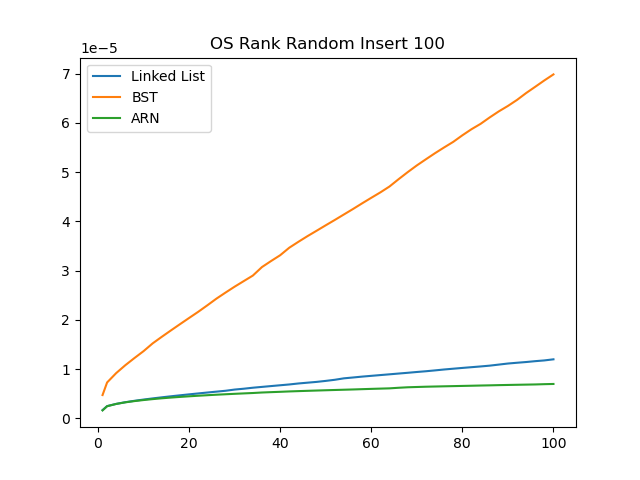
\includegraphics[width=0.8\linewidth]{Images/100/OS Rank Random Insert 100.png}
  \caption{OS Rank Random Insert 100}
  \label{fig:OS Rank Random Insert 100}
  \end{figure}
  \begin{figure}[H]
  \centering
  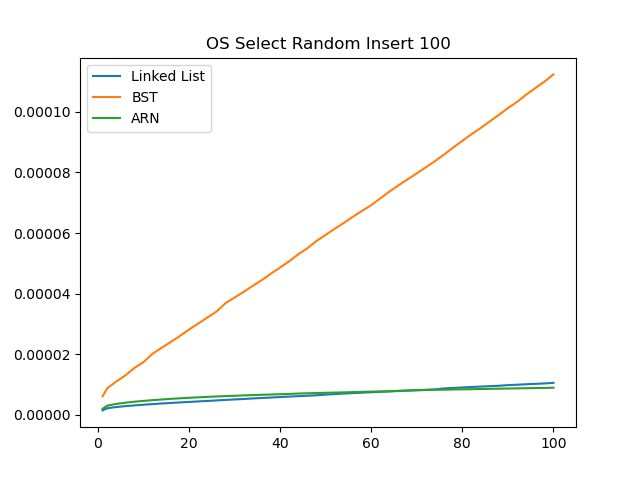
\includegraphics[width=0.8\linewidth]{Images/100/OS Select Random Insert 100.png}
  \caption{OS Select Random Insert 100}
  \label{fig:OS Select Random Insert 100}
\end{figure}
 \begin{figure}[H]
  \centering
  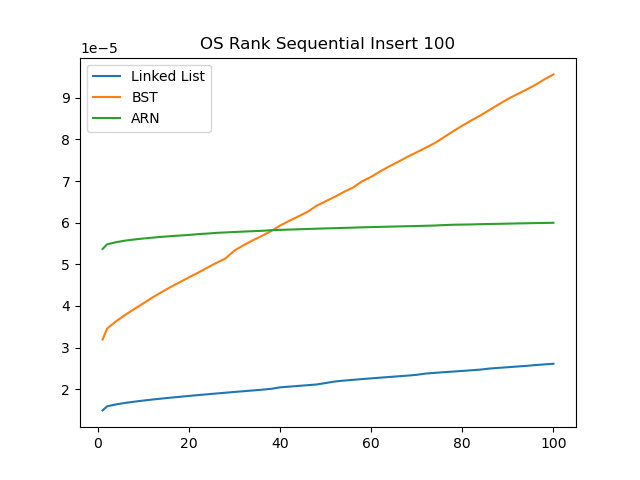
\includegraphics[width=0.8\linewidth]{Images/100/OS Rank Sequential Insert 100.png}
  \caption{OS Rank Sequential Insert 100 }
  \label{fig:OS Rank Sequential Insert 100}
\end{figure}
 \begin{figure}[H]
  \centering
  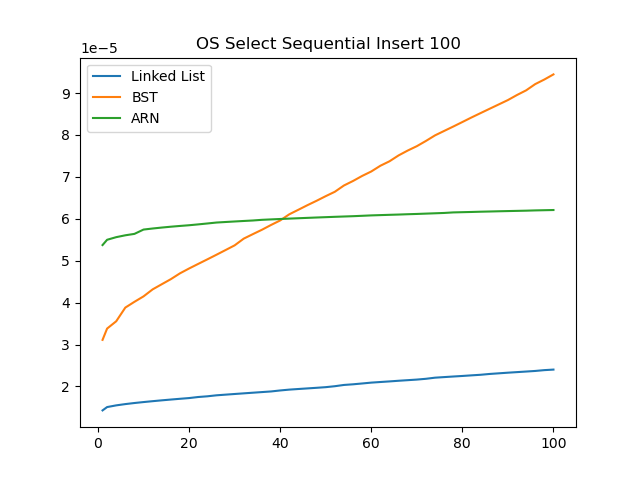
\includegraphics[width=0.8\linewidth]{Images/100/OS Select Sequential Insert 100.png}
  \caption{OS Select Sequential Insert 100 }
  \label{fig:OS Select Sequential Insert 500}
\end{figure}
 \begin{figure}[H]
  \centering
  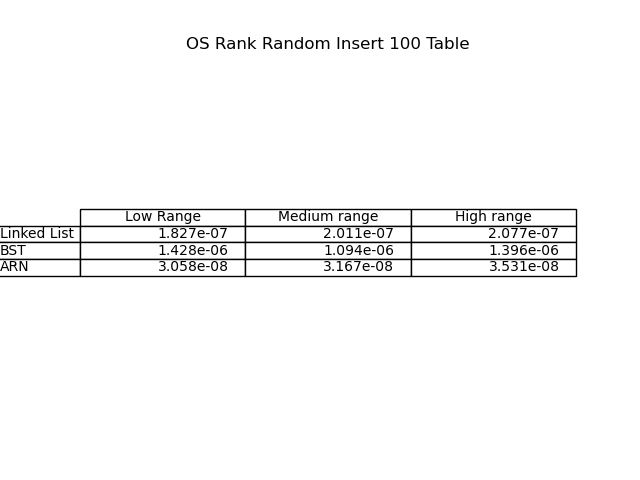
\includegraphics[width=0.8\linewidth]{Images/100/OS Rank Random Insert 100 Table.png}
  \caption{OS Rank Random Insert 100 Table }
  \label{fig:OS Rank Random Insert 100 Table}
\end{figure}
 \begin{figure}[H]
  \centering
  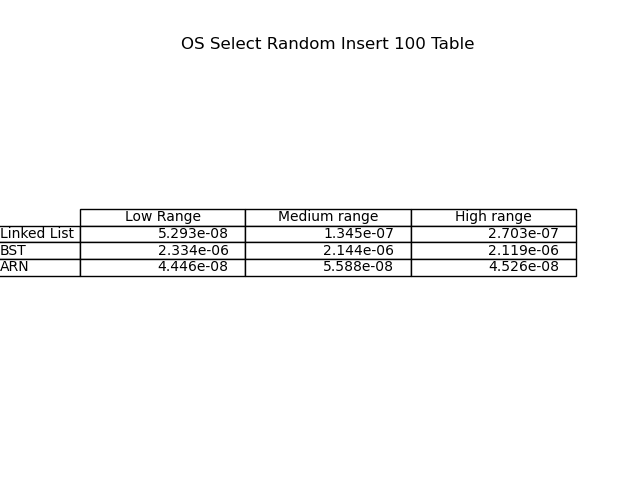
\includegraphics[width=0.8\linewidth]{Images/100/OS Select Random Insert 100 Table.png}
  \caption{OS Select Random Insert 100 Table }
  \label{fig:OS Select Random Insert 100 Table}
\end{figure}
 \begin{figure}[H]
  \centering
  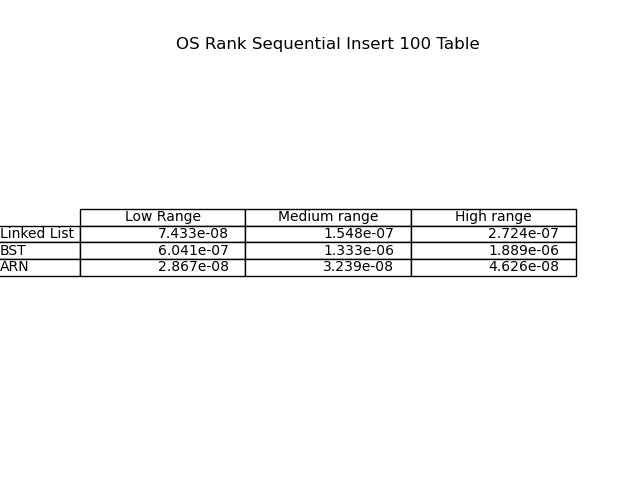
\includegraphics[width=0.8\linewidth]{Images/100/OS Rank Sequential Insert 100 Table.png}
  \caption{OS Rank Sequential Insert 100 Table }
  \label{fig:OS Rank Sequential Insert 100 Table}
\end{figure}
 \begin{figure}[H]
  \centering
  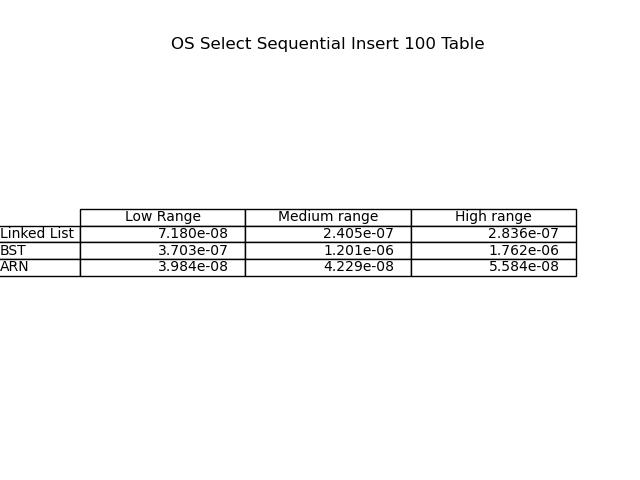
\includegraphics[width=0.8\linewidth]{Images/100/OS Select Sequential Insert 100 Table.png}
  \caption{OS Select Sequential Insert 100 Table }
  \label{fig:OS Select Sequential Insert 100 Table}
\end{figure}
\subsubsection{500 elements}

In this case, we will choose $K = 100$. 
Figures
\ref{fig:OS Rank Random Insert 500} - \ref{fig:OS Select Sequential Insert 500} confirm the hypotheses formulated in the previous case regarding the linear trend for lists and BST trees. However, it can be observed that, for larger data structures, the implementation on sorted lists is still better, but there is not a significant change in the gap between the data structures.

It can be noted that the gap in the first range of the Seuquential Inserts (\ref{fig:OS Rank Sequential Insert 500} and \ref{fig:OS Select Sequential Insert 500}) is getting narrower.

 \begin{figure}[H]
  \centering
  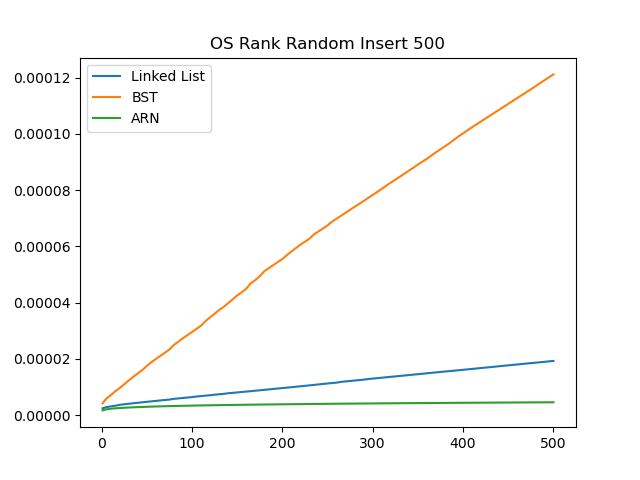
\includegraphics[width=0.8\linewidth]{Images/500/OS Rank Random Insert 500.png}
  \caption{OS Rank Random Insert 500 }
  \label{fig:OS Rank Random Insert 500}
\end{figure}
 \begin{figure}[H]
  \centering
  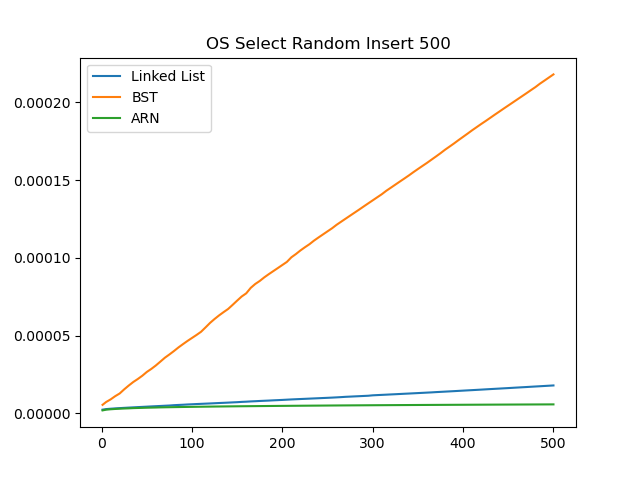
\includegraphics[width=0.8\linewidth]{Images/500/OS Select Random Insert 500.png}
  \caption{OS Select Random Insert 500 }
  \label{fig:OS Select Random Insert 500}
\end{figure}
 \begin{figure}[H]
  \centering
  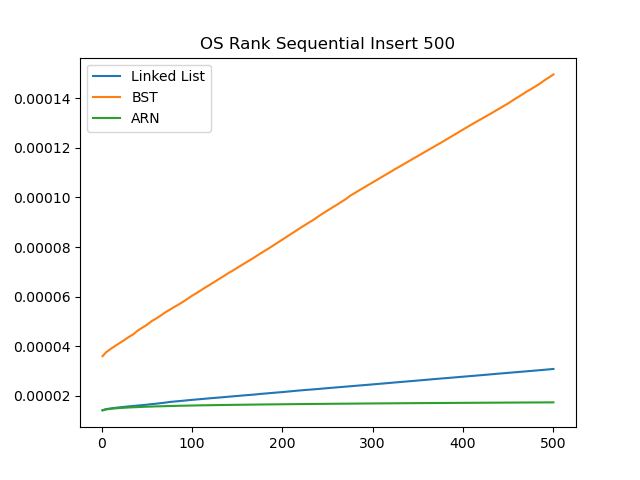
\includegraphics[width=0.8\linewidth]{Images/500/OS Rank Sequential Insert 500.png}
  \caption{OS Rank Sequential Insert 500 }
  \label{fig:OS Rank Sequential Insert 500}
\end{figure}
 \begin{figure}[H]
  \centering
  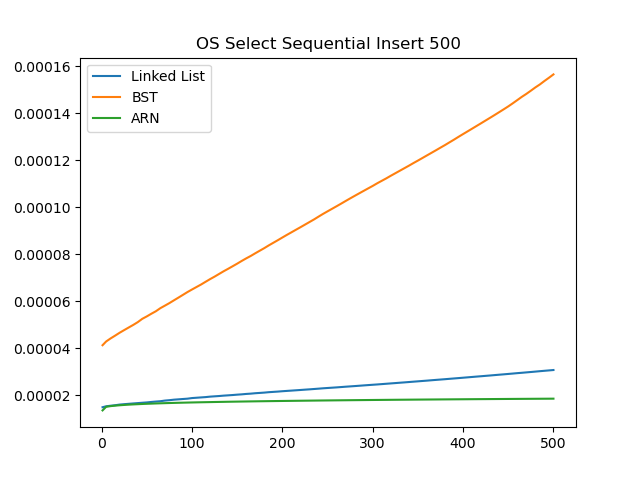
\includegraphics[width=0.8\linewidth]{Images/500/OS Select Sequential Insert 500.png}
  \caption{OS Select Sequential Insert 500 }
  \label{fig:OS Select Sequential Insert 500}
\end{figure}
 \begin{figure}[H]
  \centering
  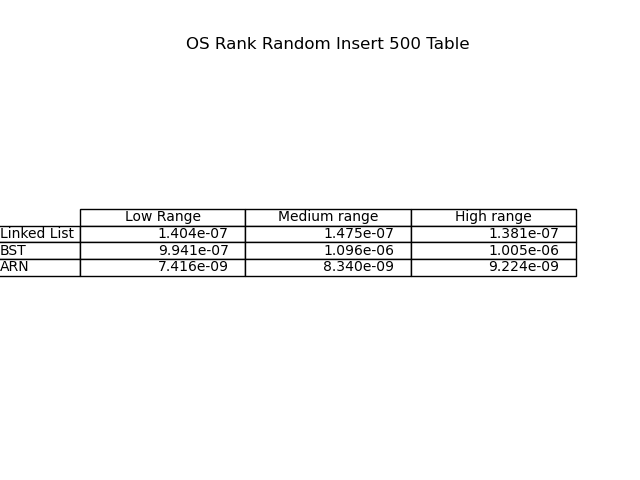
\includegraphics[width=0.8\linewidth]{Images/500/OS Rank Random Insert 500 Table.png}
  \caption{OS Rank Random Insert 500 Table }
  \label{fig:OS Rank Random Insert 500 Table}
\end{figure}
 \begin{figure}[H]
  \centering
  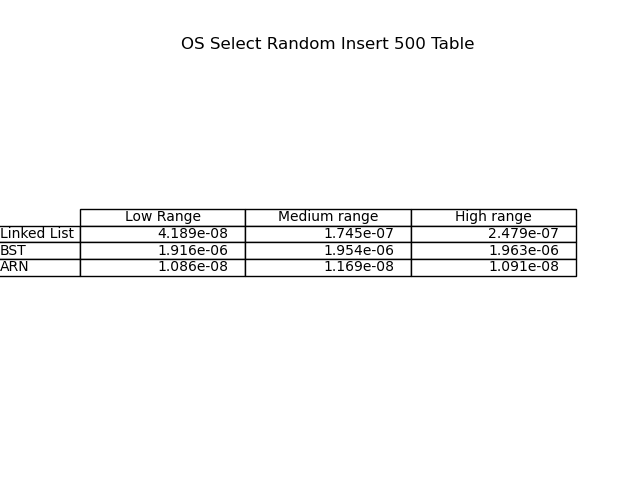
\includegraphics[width=0.8\linewidth]{Images/500/OS Select Random Insert 500 Table.png}
  \caption{OS Select Random Insert 500 Table }
  \label{fig:OS Select Random Insert 500 Table}
\end{figure}
 \begin{figure}[H]
  \centering
  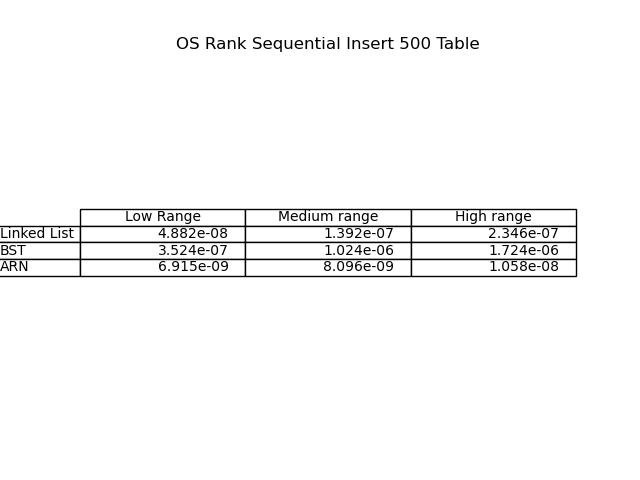
\includegraphics[width=0.8\linewidth]{Images/500/OS Rank Sequential Insert 500 Table.png}
  \caption{OS Rank Sequential Insert 500 Table }
  \label{fig:OS Rank Sequential Insert 500 Table}
\end{figure}
 \begin{figure}[H]
  \centering
  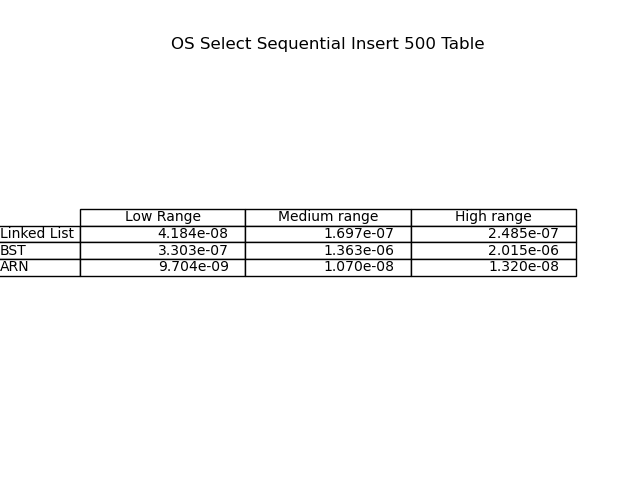
\includegraphics[width=0.8\linewidth]{Images/500/OS Select Sequential Insert 500 Table.png}
  \caption{OS Select Sequential Insert 500 Table }
  \label{fig:OS Select Sequential Insert 500 Table}
\end{figure}
\subsubsection{1000 elements}

In this case, we will also choose $K = 100$. Having established in previous cases the complexity of the different implementations of the OS algorithms, in this instance, we will only comment on the graphs that allow us to compare them. Indeed, by observing figures \ref{fig:OS Rank Random Insert 1000}-\ref{fig:OS Select Sequential Insert 1000}, it can be noted that, for large data structures, the OS algorithms perform in the same way as the previous test.

Now let's analyze the average execution times for the three ranges of indices/nodes input to the OS Select and OS Rank functions, as observable in \ref{fig:OS Rank Random Insert 1000 Table}-\ref{fig:OS Select Sequential Insert 1000 Table}. 

In the case of sorted lists, we notice that the algorithms are faster in the lower range and slower in the higher range, because the indices/nodes are searched starting from the first ones. Few differences occur in the case of random insertion, since, being the list sorted, the order of the nodes in the list is not influenced by their insertion order.

As for BST trees with sequential insertion, we can make a similar observation to that made for lists, the implementations of the OS algorithms on these data structures are based on the same fundamental idea (we can also think that a completely unbalanced binary tree becomes a list)

As noted in the last test, the gap in the Sequential Inserts, as the number of elements grows, gets narrower.


 \begin{figure}[H]
  \centering
  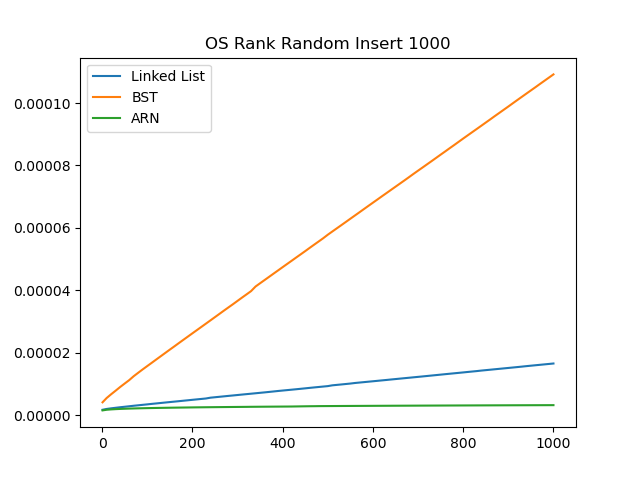
\includegraphics[width=0.8\linewidth]{Images/1000/OS Rank Random Insert 1000.png}
  \caption{OS Rank Random Insert 1000 }
  \label{fig:OS Rank Random Insert 1000}
\end{figure}
 \begin{figure}[H]
  \centering
  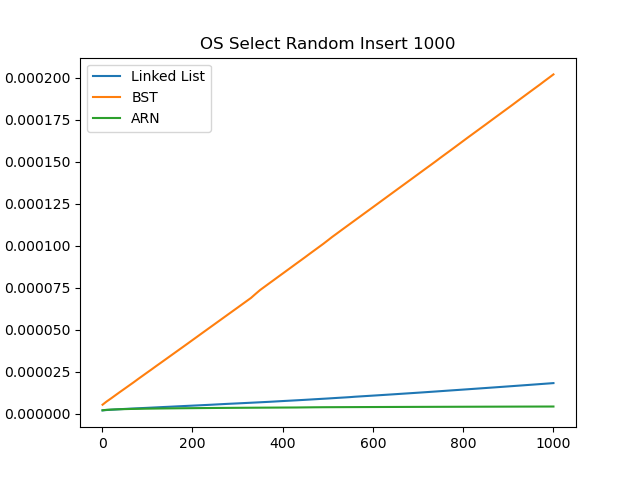
\includegraphics[width=0.8\linewidth]{Images/1000/OS Select Random Insert 1000.png}
  \caption{OS Select Random Insert 1000 }
  \label{fig:OS Select Random Insert 1000}
\end{figure}
 \begin{figure}[H]
  \centering
  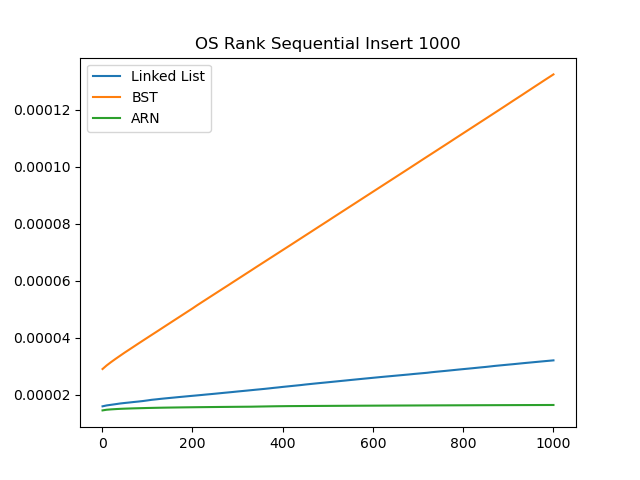
\includegraphics[width=0.8\linewidth]{Images/1000/OS Rank Sequential Insert 1000.png}
  \caption{OS Rank Sequential Insert 1000 }
  \label{fig:OS Rank Sequential Insert 1000}
\end{figure}
 \begin{figure}[H]
  \centering
  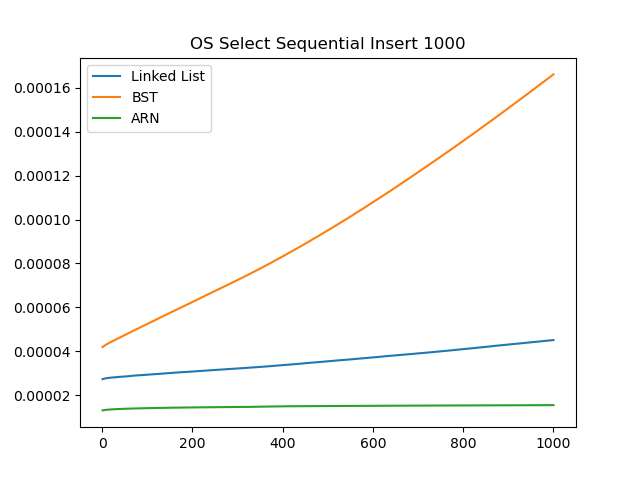
\includegraphics[width=0.8\linewidth]{Images/1000/OS Select Sequential Insert 1000.png}
  \caption{OS Select Sequential Insert 1000 }
  \label{fig:OS Select Sequential Insert 1000}
\end{figure}
 \begin{figure}[H]
  \centering
  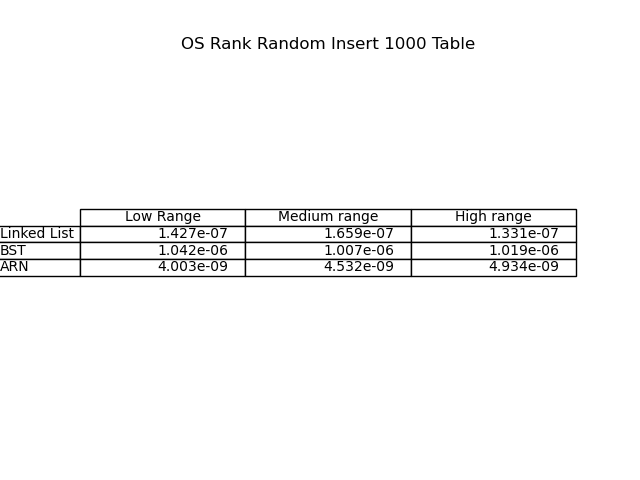
\includegraphics[width=0.8\linewidth]{Images/1000/OS Rank Random Insert 1000 Table.png}
  \caption{OS Rank Random Insert 1000 Table }
  \label{fig:OS Rank Random Insert 1000 Table}
\end{figure}
 \begin{figure}[H]
  \centering
  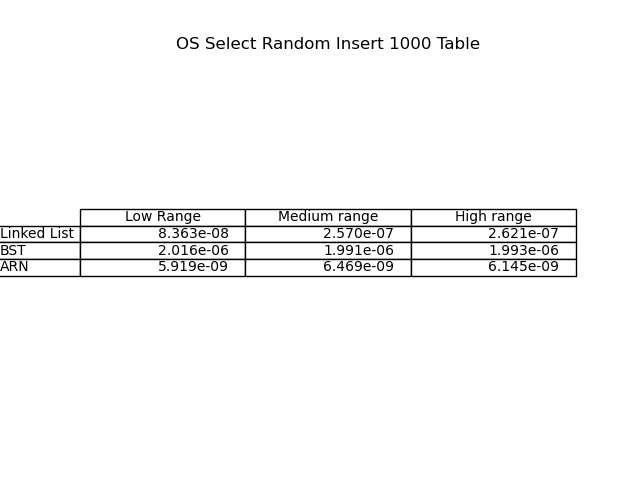
\includegraphics[width=0.8\linewidth]{Images/1000/OS Select Random Insert 1000 Table.png}
  \caption{OS Select Random Insert 1000 Table }
  \label{fig:OS Select Random Insert 1000 Table}
\end{figure}
 \begin{figure}[H]
  \centering
  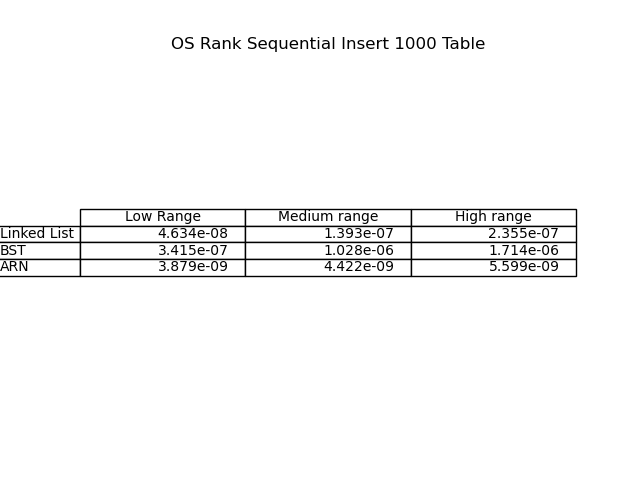
\includegraphics[width=0.8\linewidth]{Images/1000/OS Rank Sequential Insert 1000 Table.png}
  \caption{OS Rank Sequential Insert 1000 Table }
  \label{fig:OS Rank Sequential Insert 1000 Table}
\end{figure}
 \begin{figure}[H]
  \centering
  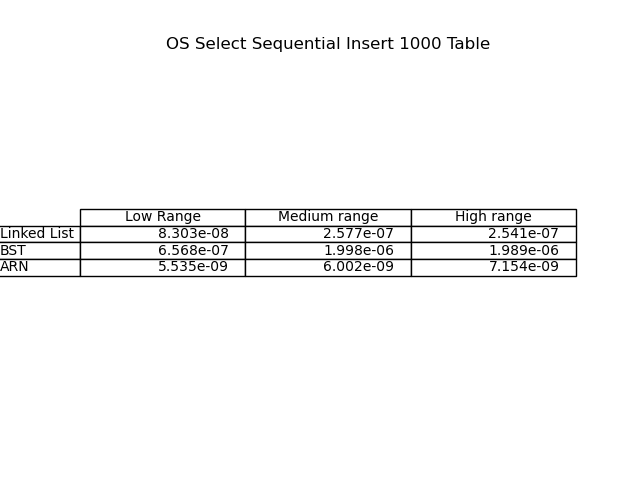
\includegraphics[width=0.8\linewidth]{Images/1000/OS Select Sequential Insert 1000 Table.png}
  \caption{OS Select Sequential Insert 1000 Table }
  \label{fig:OS Select Sequential Insert 1000 Table}
\end{figure}
\subsubsection{1500 elements}
For this last test, it was necessary to grant VisualStudio Code the use of more memory to handle the high number of recursive calls. Again, we will only observe the graphs that compare the performance on different data structures(\ref{fig:OS Rank Random Insert 1500} - \ref{fig:OS Select Sequential Insert 1500}), printed by choosing $K = 300$. These last tests only confirm the observations made in previous cases, showing how the implementation on both the data structures share the same trend, since there is no significant change in the gap between the two.
 \begin{figure}[H]
  \centering
  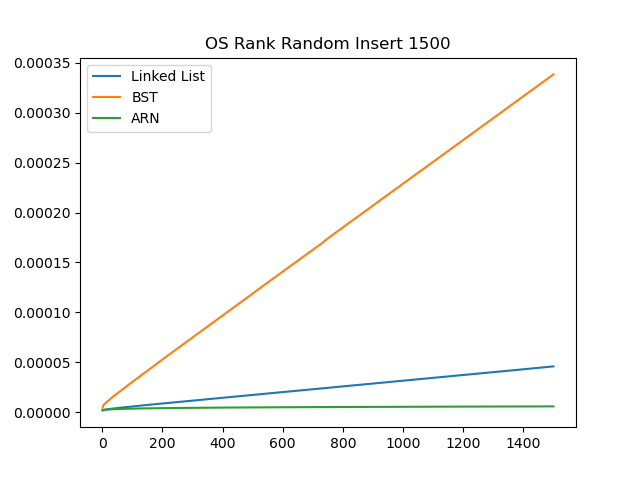
\includegraphics[width=0.8\linewidth]{Images/1500/OS Rank Random Insert 1500.png}
  \caption{OS Rank Random Insert 1500 }
  \label{fig:OS Rank Random Insert 1500}
\end{figure}
 \begin{figure}[H]
  \centering
  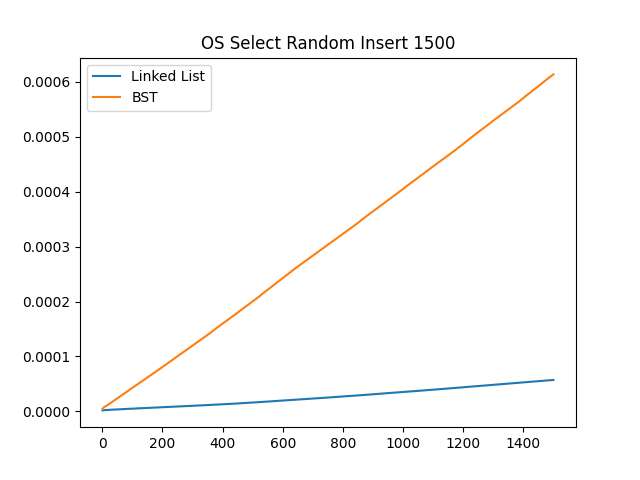
\includegraphics[width=0.8\linewidth]{Images/1500/OS Select Random Insert 1500.png}
  \caption{OS Select Random Insert 1500 }
  \label{fig:OS Select Random Insert 1500}
\end{figure}
 \begin{figure}[H]
  \centering
  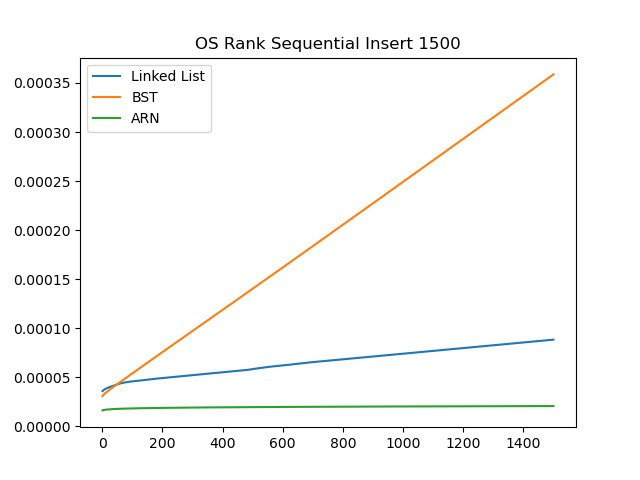
\includegraphics[width=0.8\linewidth]{Images/1500/OS Rank Sequential Insert 1500.png}
  \caption{OS Rank Sequential Insert 1500 }
  \label{fig:OS Rank Sequential Insert 1500}
\end{figure}
 \begin{figure}[H]
  \centering
  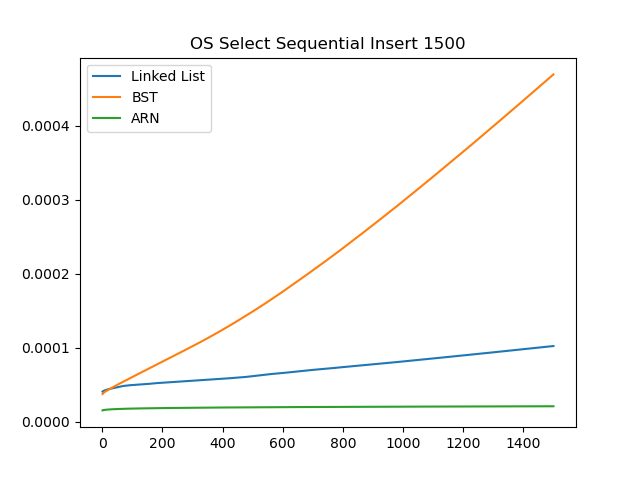
\includegraphics[width=0.8\linewidth]{Images/1500/OS Select Sequential Insert 1500.png}
  \caption{OS Select Sequential Insert 1500 }
  \label{fig:OS Select Sequential Insert 1500}
\end{figure}
 \begin{figure}[H]
  \centering
  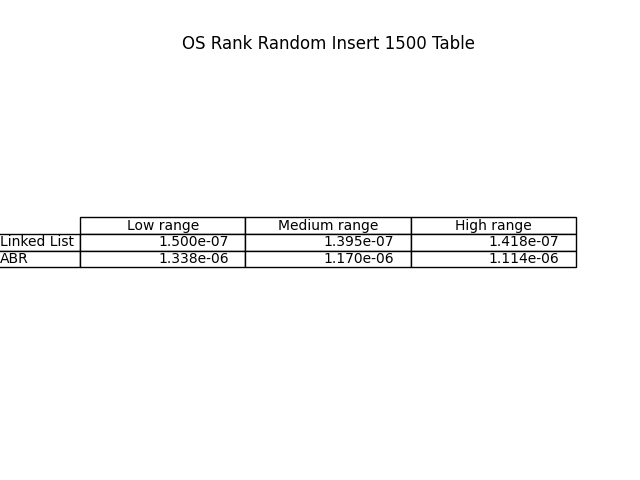
\includegraphics[width=0.8\linewidth]{Images/1500/OS Rank Random Insert 1500 Table.png}
  \caption{OS Rank Random Insert 1500 Table }
  \label{fig:OS Rank Random Insert 1500 Table}
\end{figure}
 \begin{figure}[H]
  \centering
  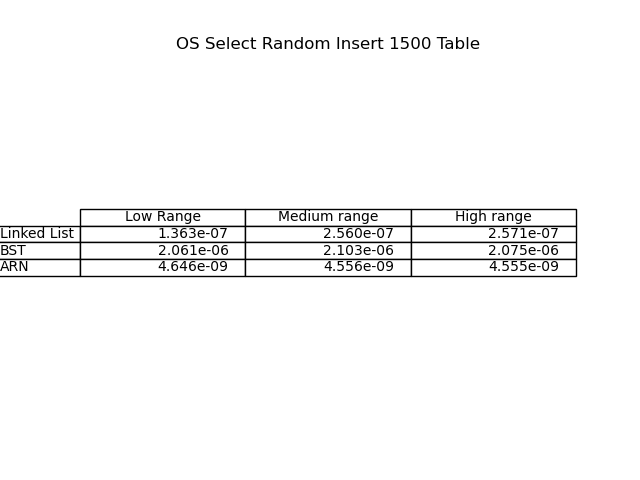
\includegraphics[width=0.8\linewidth]{Images/1500/OS Select Random Insert 1500 Table.png}
  \caption{OS Select Random Insert 1500 Table }
  \label{fig:OS Select Random Insert 1500 Table}
\end{figure}
 \begin{figure}[H]
  \centering
  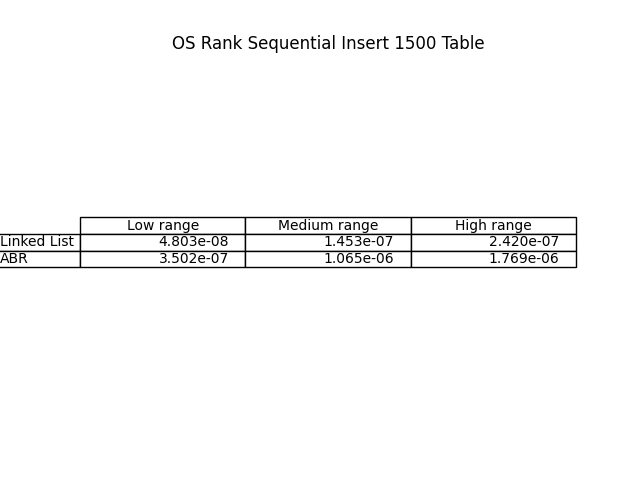
\includegraphics[width=0.8\linewidth]{Images/1500/OS Rank Sequential Insert 1500 Table.png}
  \caption{OS Rank Sequential Insert 1500 Table }
  \label{fig:OS Rank Sequential Insert 1500 Table}
\end{figure}
 \begin{figure}[H]
  \centering
  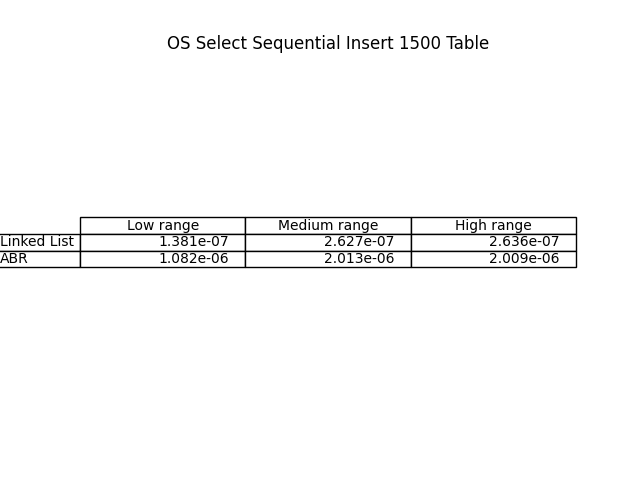
\includegraphics[width=0.8\linewidth]{Images/1500/OS Select Sequential Insert 1500 Table.png}
  \caption{OS Select Sequential Insert 1500 Table }
  \label{fig:OS Select Sequential Insert 1500 Table}
\end{figure}
\section{Test discussion and conclusions}
The test results reaffirm the hypothesis:

Sorted lists are a valid choice for small-sized data structures, especially fast when dealing with the first elements of the list.
Finally, the implementation for BST without the size attribute has proven to be the least effective, as the absence of such a parameter makes it impossible to exploit the potential of the data structure and instead forces a much less elaborate approach similar to that adopted for lists. Performance on BSTs is significantly worse due to the time spent descending and ascending the tree through recursive calls, and even when the tree is more balanced, the performance improvement is relative.

In terms of performance concerning the number of elements, however, both implementations have not undergone significant changes to highlight further differences if we only consider the last elements, while the data structures share the same results, with a bigger set of elements, with the first few elements. 
\end{document}

